\chapter{FEL theory: statistical optics perspective}
\label{chapter:FEL theory}


A free-electron laser can be generally considered as an amplifier and its coherence properties can be characterized from this point of view. 

\begin{figure*}[h!]
	\centering
    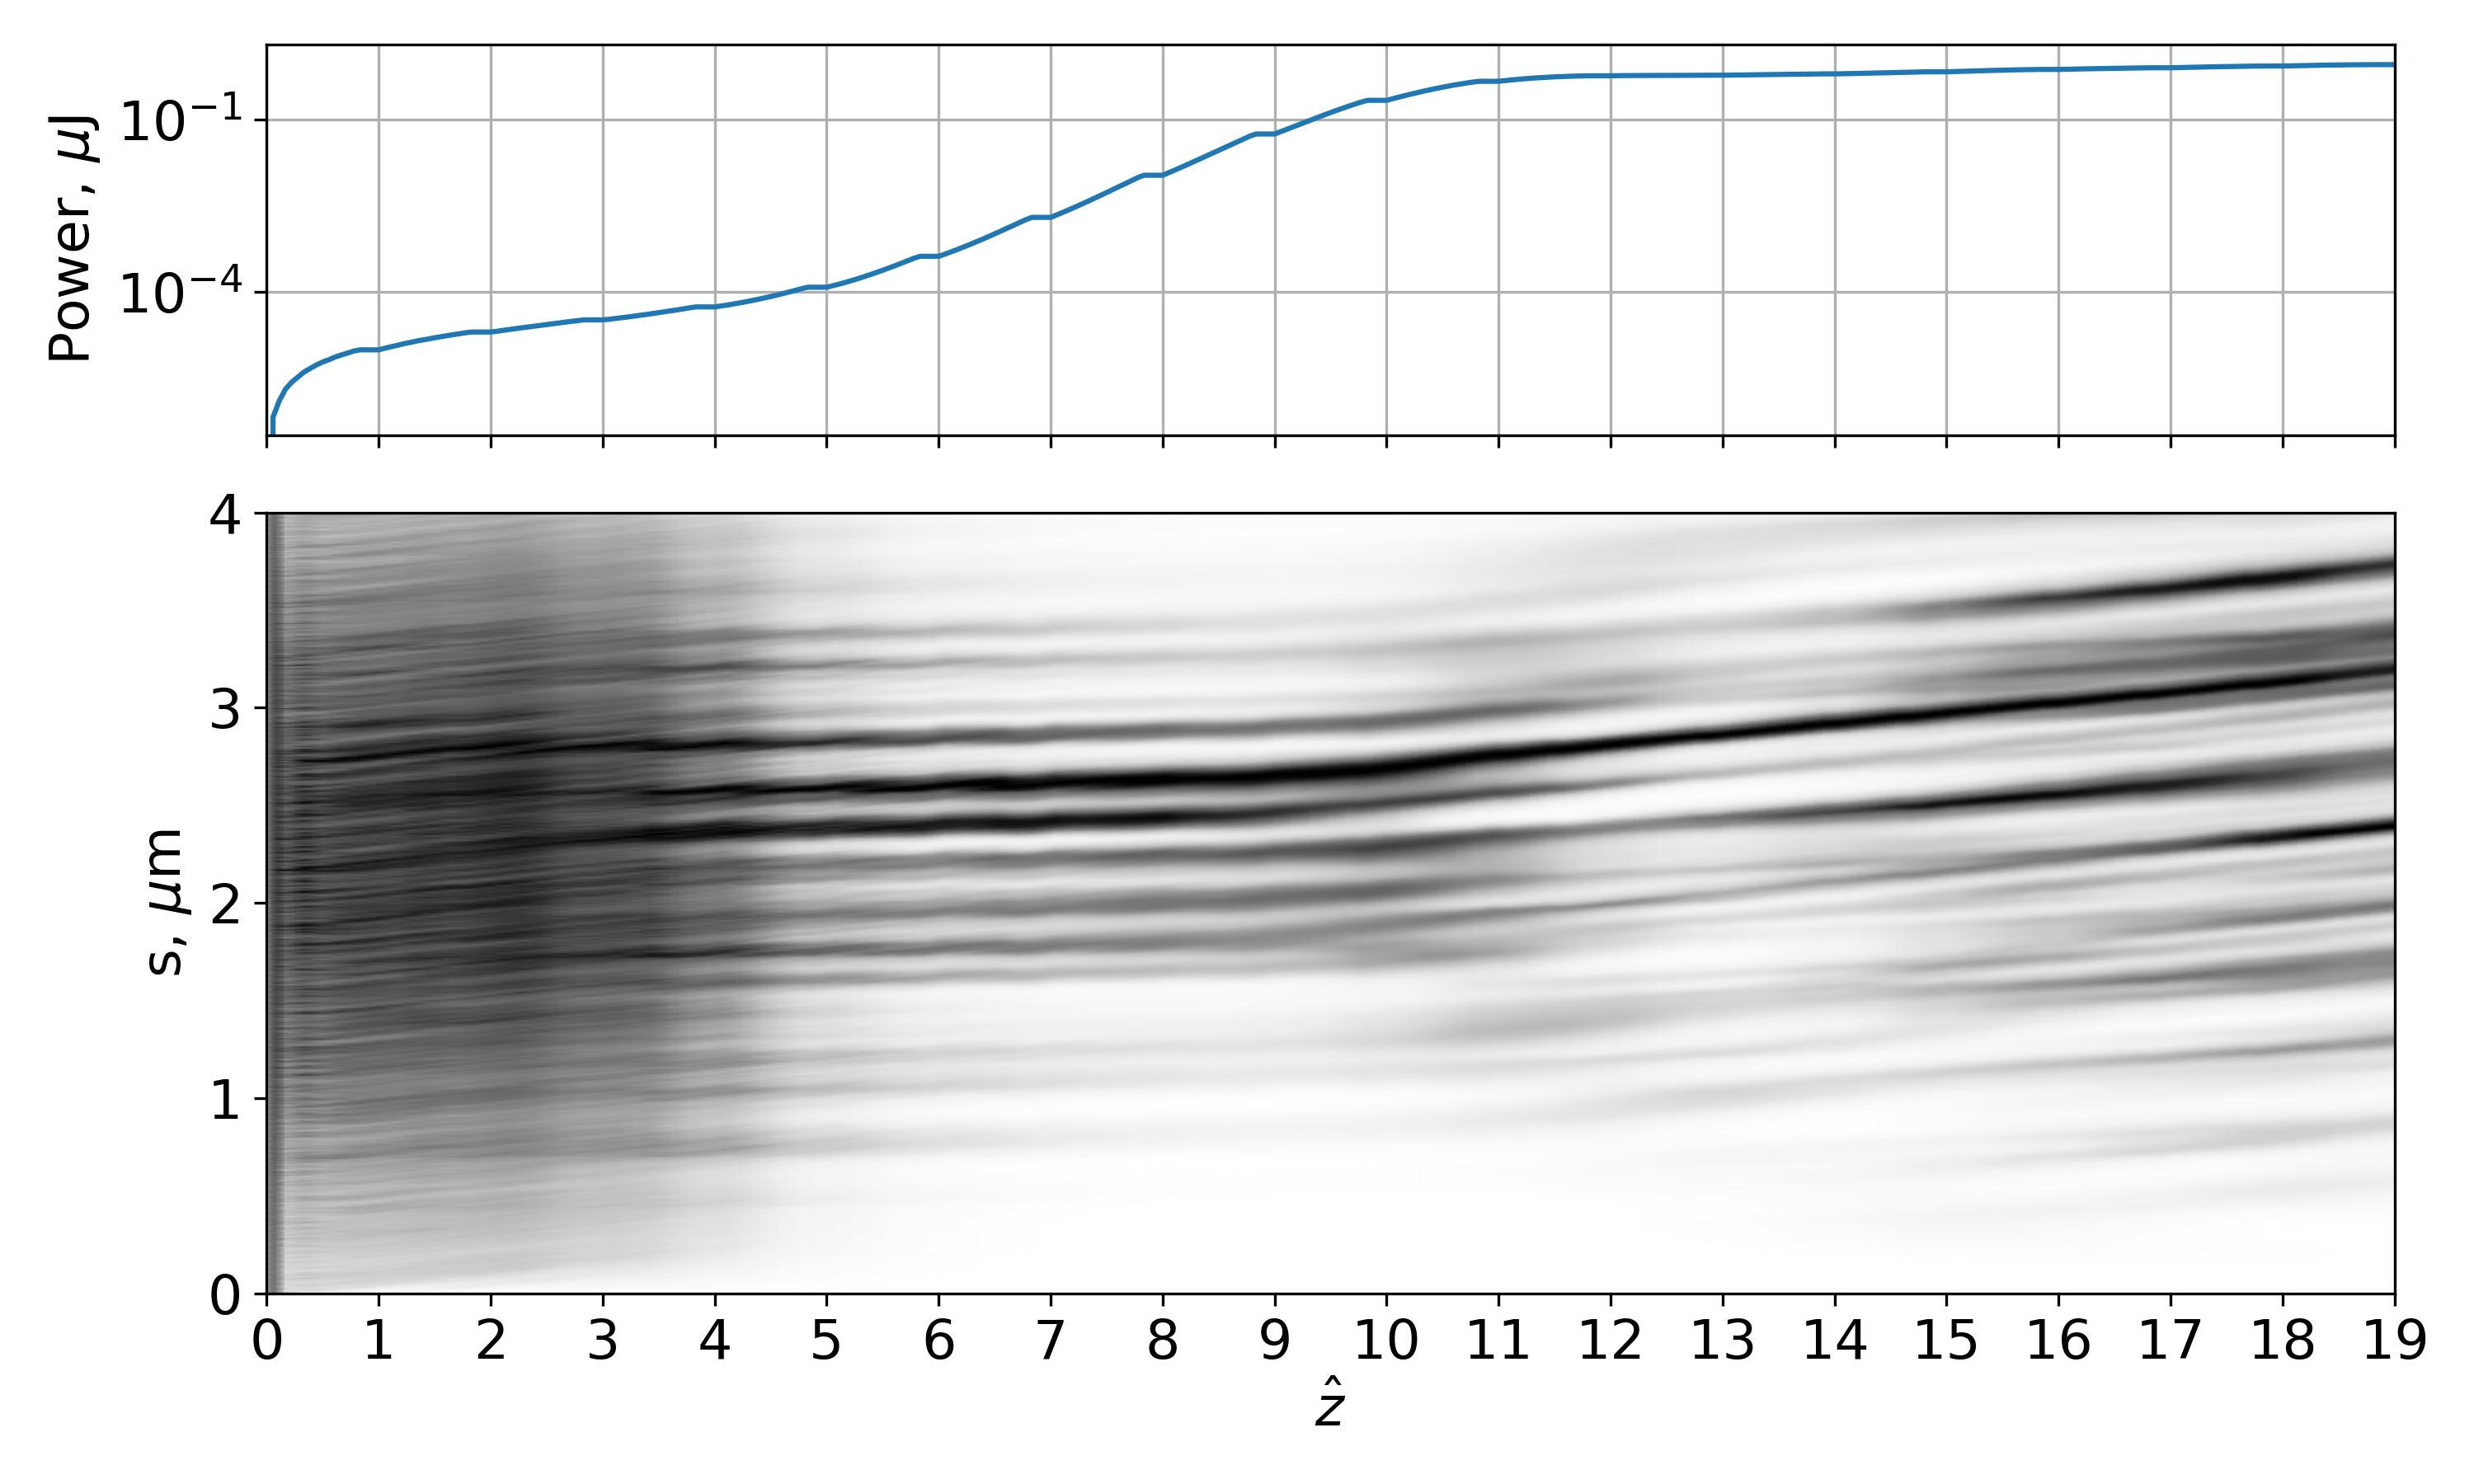
\includegraphics[width=0.95\linewidth]{content/images/4_FEL_Theory/evo_spikes.png}
\captionsetup{justification=centering}
    \caption{}
    \label{fig:pole}
\end{figure*}

\begin{figure*}[h!]
	\centering
    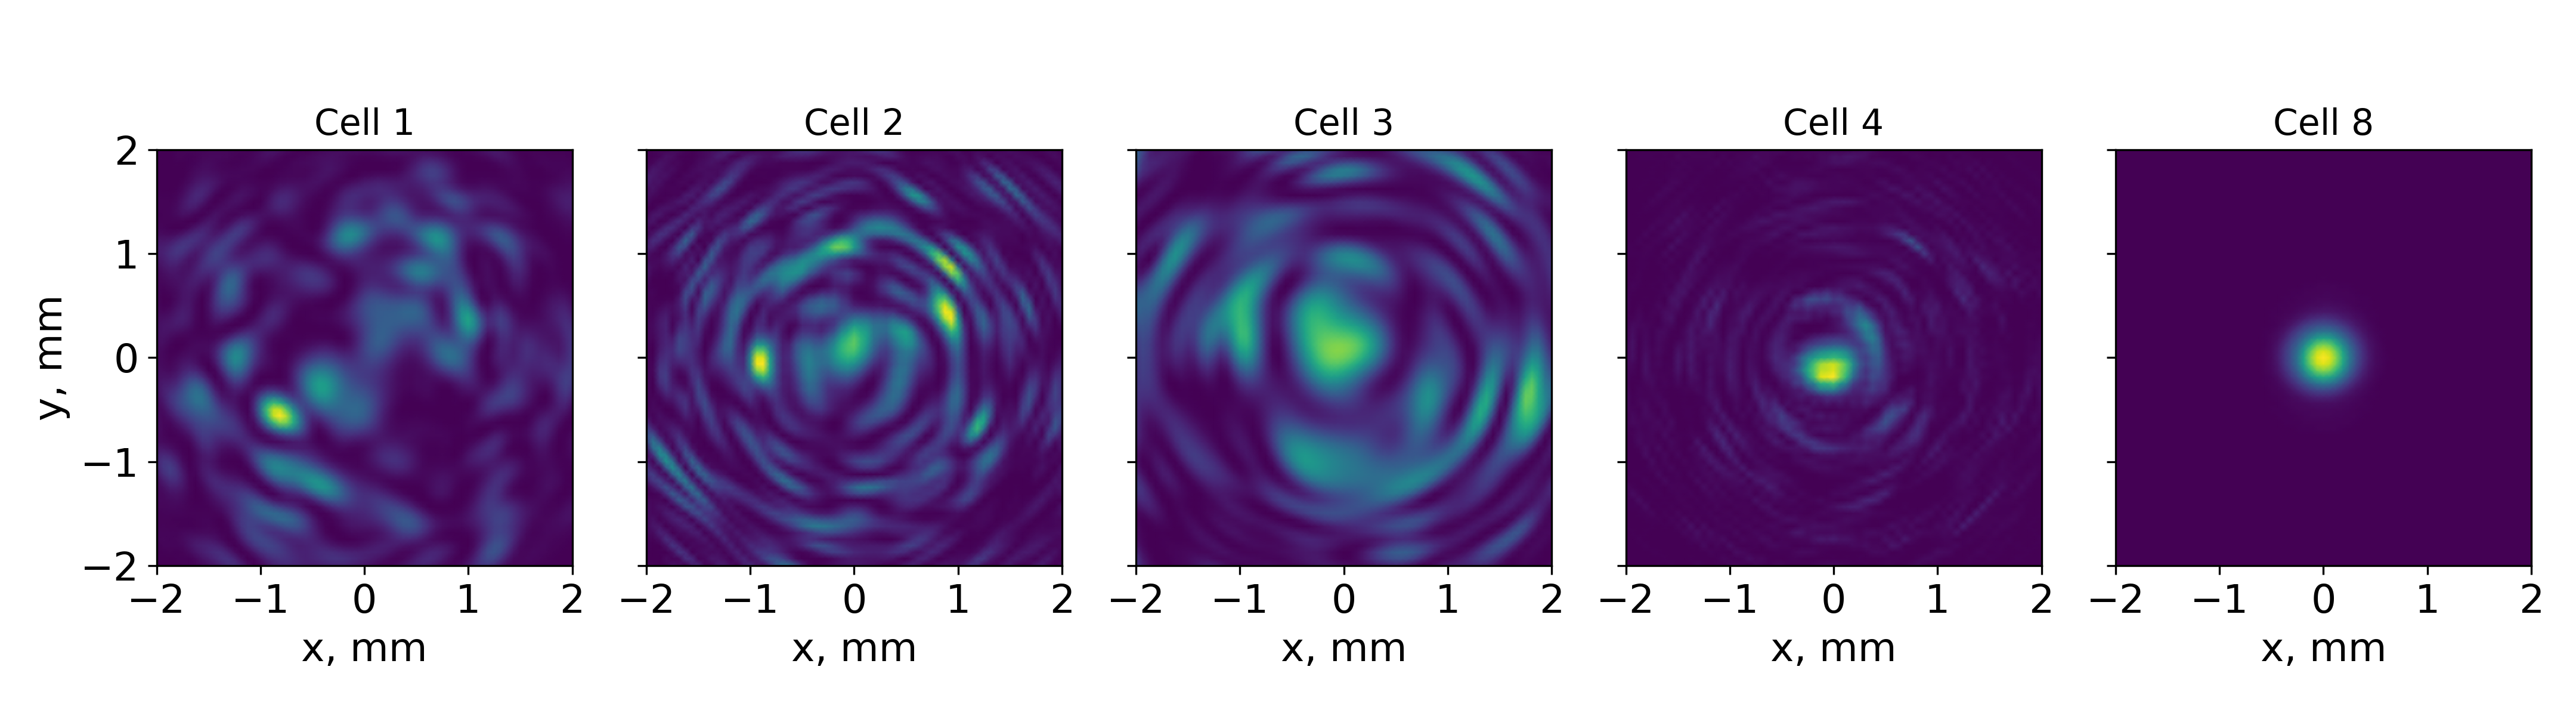
\includegraphics[width=1.1\linewidth]{content/images/4_FEL_Theory/transverse_modes.png}
    \captionsetup{justification=centering}
    \caption{}
    \label{fig:pole}
\end{figure*}
\rr{write about Gaussian statistics}\\
\rr{write about chirps}

\subsection{Heuristic approach: quasi- homogeneous/stationary source with chirps}
    Here I start with definition of the Wigner function distribution 
    \begin{align}
        \mathcal{W}(\bar{t}, \bar{\omega}) = \int \limits_{-\infty}^{\infty} \Tilde{\Gamma}(\bar{\omega}, \Delta \omega) e^{-i\Delta \omega \bar{t}}d(\Delta \omega)
    \end{align}
    One may notice that for a source that can be represented $\Tilde{\Gamma}(\omega, \Delta \omega) = f_{\omega}(\Delta \omega)\bar{I}(\bar{\omega})$ the integral factorises and as a result $\mathcal{W}(t, \omega)$ can be written as the following:
    \begin{align}
        \mathcal{W}(\bar{t}, \bar{\omega}) = \bar{I}(\bar{\omega}) \int \limits_{-\infty}^{\infty} f_{\omega}(\Delta \omega) e^{-i\Delta \omega \bar{t}}d(\Delta \omega) = \bar{I}(\bar{\omega}) I(\bar{t})
    \end{align}
    This representation hints that \rr{previous SERVAL formula} is actually represent factorized representation (by in spatial domain) and this equation can be modernised for use of the Wigner function:
    \begin{align}
    	\phi(\bar{\omega}) = \int \limits_{-\infty}^{\infty} \sqrt{\mathcal{W}(\bar{\omega}, \bar{t})} \mathcal{N}(\bar{t}) e^{i \bar{\omega} \bar{t}} d\bar{t}.
    	\label{Eq:Field_Wigner}
    \end{align}
    \subsection{SERVAL2 paper}
    \includepdf[pages=-]{content/papers/SERVAL2.pdf}


\section{Radiation at harmonics paper}
\includepdf[pages=-]{content/papers/attoharm.pdf}
